% =============================================================
%  PART B — Seasonal UHI from MODIS
%  Person U  ·  Mumbai UHI Assignment
% =============================================================
%  MERGE NOTE FOR M: compiles standalone, or \input{} into the
%  combined report. No \section numbers are hard-coded.
%
%  \TODO{...} marks what still needs writing. All numbers are
%  filled in from the Earth Engine output; what remains is the
%  interpretation, which has to be written by hand.
% =============================================================

\documentclass[11pt,a4paper]{article}

\usepackage[margin=1in]{geometry}
\usepackage{booktabs}
\usepackage{graphicx}
\usepackage{amsmath}
\usepackage{siunitx}
\usepackage[hidelinks]{hyperref}
\usepackage{xcolor}

% \long so a TODO block may contain paragraph breaks and lists.
\newcommand\TODO{}
\long\def\TODO#1{{\color{red}[TODO: #1]}}

\sisetup{detect-all, per-mode=symbol}
\graphicspath{{figures/}}

\title{Characterising the Urban Heat Island of Mumbai\\
       \large Part B — Seasonal UHI from MODIS}
\author{\TODO{Name} (\TODO{Roll No.})}
\date{\today}

\begin{document}
\maketitle

% =============================================================
\section{Data and platform}
% =============================================================

\subsection{Product}

Seasonal LST comes from the MODIS eight-day composites,
\texttt{MODIS/061/MOD11A2} (Terra) and \texttt{MODIS/061/MYD11A2}
(Aqua), both at \SI{1}{\kilo\metre}. These are Collection 6.1
split-window retrievals with land-cover-based emissivity.

We used the eight-day product rather than the daily one
(\texttt{MOD11A1}/\texttt{MYD11A1}) because the daily product leaves
every cloud gap to be handled by hand, and Mumbai has four months of
near-continuous monsoon cloud. The eight-day product applies a
consistent clear-sky selection instead. The cost is that it hides how
few days actually contributed, which matters here and is measured in
Section~\ref{sec:sampling}.

\subsection{Terra and Aqua}

We used both platforms rather than picking one.

Terra crosses at about \texttt{10:30} and \texttt{22:30} local solar
time. Aqua crosses at about \texttt{13:30} and \texttt{01:30}. Terra's
morning pass is close to Landsat~8's (\(\approx\)\texttt{10:30}), so
the Terra daytime numbers are the ones that can be compared against
Part~A. Aqua sits nearer the daily maximum and the pre-dawn minimum,
so it gives a better estimate of the true extremes.

Using both means the seasonal cycle can be reported at the daily
extremes while still keeping a like-for-like row for the Landsat
comparison. The Terra--Aqua gap within a season is also useful on its
own: it isolates time of day from season.

Rather than trusting the nominal crossing times we extracted the
actual mean observation time from the \texttt{Day\_view\_time} and
\texttt{Night\_view\_time} bands. Over the urban zone these came out
at \textbf{10:38} and \textbf{22:14} for Terra, \textbf{13:28} and
\textbf{01:52} for Aqua --- close enough to the nominal times that no
correction is needed, and Terra's morning pass sits within about eight
minutes of Landsat's.

% =============================================================
\section{Season definition}
% =============================================================

Seasons follow the India Meteorological Department's four-season
classification \citep{imd_seasons}:

\begin{table}[htbp]
\centering
\begin{tabular}{lll}
\toprule
\textbf{Season} & \textbf{Months} & \textbf{Role here} \\
\midrule
Winter                & January--February  & Seasonal contrast \\
Pre-monsoon (summer)  & March--May         & Seasonal contrast \\
Southwest monsoon     & June--September    & Seasonal contrast \\
Post-monsoon          & October--December  & Landsat comparison \\
\bottomrule
\end{tabular}
\caption{IMD seasonal classification. All four were computed.}
\label{tab:seasons}
\end{table}

\paragraph{Why all four.}
The brief asks for two or three seasons, and the first three cover the
full range of surface moisture and insolation in Mumbai. We added
post-monsoon because the Landsat pair in Part~A was acquired on
8--9~October~2015, which falls in it. Without that season the
cross-sensor comparison in Section~\ref{sec:comparison} would have had
to compare across sensor and season at once.

\paragraph{Why IMD and not DJF/MAM/JJA.}
December--January--February for winter is a mid-latitude convention
and does not describe a tropical monsoon coast. Mumbai's year is set
by the onset and withdrawal of the southwest monsoon, not by the
solstices. Two things follow. December still carries post-monsoon soil
moisture and is not thermally like January, so IMD puts it in
post-monsoon instead. And none of the IMD seasons crosses a calendar
year, so each year gives exactly one clean instance of each season ---
which is what makes the year-by-year analysis in
Section~\ref{sec:interannual} work at all. A DJF winter would straddle
two years and force an arbitrary choice about which year each December
belongs to.

\paragraph{Climatological basis.}
\TODO{Two or three sentences on Mumbai's climate with a citation:
mean monthly temperature and rainfall, and the normal onset and
withdrawal dates of the monsoon. IMD Climatological Tables or the
IMD Mumbai regional page. This is what turns the season definition
from an assertion into a defended choice, so it needs a real source.}

% =============================================================
\section{Method}
% =============================================================

\subsection{Study area and zones}

The area of interest is the GADM v4.1 level-2 boundary for Mumbai
\citep{gadm}, supplied as an ESRI shapefile in EPSG:4326 (WGS~84
geographic). No reprojection was applied; Earth Engine works in
EPSG:4326 internally, and all areas were computed on the ellipsoid
rather than in projected units. The polygon measures
\SI{481.56}{\kilo\metre\squared} by ellipsoidal calculation, against
the \SI{480.10}{\kilo\metre\squared} recorded in the file's own
\texttt{area\_km2} attribute; the \SI{1.5}{\kilo\metre\squared}
difference is a consequence of the two methods, not a discrepancy in
the data.

Zones are defined from ESA WorldCover v200 (2021) \citep{worldcover}:

\begin{itemize}
  \item \textbf{Urban} --- built-up (class~50) inside the boundary.
        Area \SI{204.72}{\kilo\metre\squared}.
  \item \textbf{Rural} --- tree cover, shrubland, grassland, cropland
        and bare/sparse (classes 10, 20, 30, 40, 60) in a ring from
        \SI{5}{\kilo\metre} to \SI{20}{\kilo\metre} beyond the
        boundary. Area \SI{962.13}{\kilo\metre\squared}.
\end{itemize}

The \SI{5}{\kilo\metre} inner gap keeps the peri-urban fringe and the
city's own thermal plume out of the reference. The outer limit of
\SI{20}{\kilo\metre} keeps the ring within the same coastal climate.
Both limits are varied in Section~\ref{sec:ringsens}.

\begin{figure}[htbp]
\centering
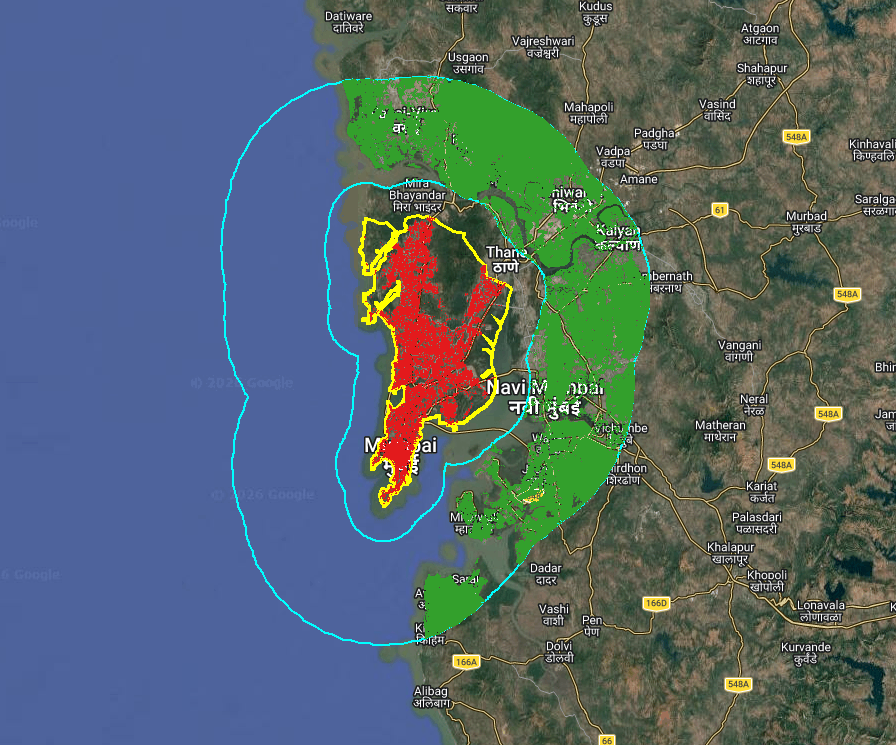
\includegraphics[width=0.78\textwidth]{zones_map_gee.png}
\caption{Urban zone (red), rural ring (green), district boundary
(yellow) and the outer edge of the ring (cyan). The western half of
the ring is open sea and drops out entirely once water is excluded.}
\label{fig:zones}
\end{figure}

\subsection{Water and wetland exclusion}
\label{sec:waterexcl}

Permanent water (class~80) was removed from both zones. Herbaceous
wetland (90) and mangrove (95) were also removed from the rural
reference, because Mumbai's creeks are mangrove-lined and tidally
inundated, so those surfaces behave thermally like water rather than
land.

This matters more here than it would inland. The rural ring covers
\SI{2785.04}{\kilo\metre\squared} of geometric area, but

\begin{table}[htbp]
\centering
\begin{tabular}{lrr}
\toprule
\textbf{Cover} & \textbf{Area (\si{\kilo\metre\squared})} & \textbf{Share} \\
\midrule
Permanent water (80)        & 1534.65 & 55.1\,\% \\
Wetland and mangrove (90, 95) &   73.64 &  2.6\,\% \\
Built-up (50)               &  214.63 &  7.7\,\% \\
Usable rural cover          &  962.13 & 34.5\,\% \\
\midrule
Ring total                  & 2785.04 & 100\,\% \\
\bottomrule
\end{tabular}
\caption{What the rural ring is made of. Over half is sea.}
\label{tab:ringcomp}
\end{table}

More than half the ring is sea. The reason for removing it is
physical, not conventional: water has very high heat capacity and
thermal inertia, so its surface temperature barely moves over the
diurnal cycle while land swings widely. Leaving it in would anchor the
rural mean to a surface that cannot respond to the forcing being
measured.

The resulting bias would also change sign between day and night. The
sea is cooler than land by day, which would pull the rural mean down
and inflate daytime UHI; it is warmer than land by night, which would
push the rural mean up and suppress night-time UHI. We measured this
rather than assuming it --- see Section~\ref{sec:watertest}.

\subsection{Quality screening}
\label{sec:qc}

Pixels were screened on \texttt{QC\_Day} and \texttt{QC\_Night}. Two
conditions were required: mandatory QA (bits 0--1) of 0 or 1, i.e.\
not cloud-flagged and not otherwise unproduced; and LST error (bits
6--7) of 2 or better, i.e.\ an average retrieval error at or below
\SI{3}{\kelvin}.

The eight-day product is already cloud-screened, so this is not cloud
masking. It removes retrievals produced under marginal conditions with
large stated errors, which in a monsoon climate cluster in exactly the
season of most interest.

A stricter setting (mandatory QA $=0$ and LST error
$\leq\,$\SI{2}{\kelvin}) was tried first and emptied some night zones
entirely, which produced null zonal means. The relaxed setting was
used for all results reported here. Pixel counts under the relaxed
setting are given in Table~\ref{tab:headline} and never fall below 239
urban and 917 rural.

\subsection{Scaling and statistics}

LST bands were multiplied by \num{0.02} to give kelvin, then
\SI{273.15}{\kelvin} subtracted for degrees Celsius. View-time bands
were multiplied by \num{0.1} for local solar hours.

For each platform, mode and season, all qualifying composites from
2019--2023 were averaged per pixel. Zonal means were taken with
\texttt{reduceRegion} at \SI{1000}{\metre} --- the native MODIS grid
spacing, so no resampling happens before the statistics. UHI intensity
is

\begin{equation}
  \mathrm{UHI} = \overline{T_{\mathrm{urban}}} - \overline{T_{\mathrm{rural}}}
\end{equation}

At \SI{1}{\kilo\metre} the urban zone holds 241 valid pixels and the
rural zone 917--1055 depending on season and mode. The urban count is
the binding constraint on precision and is discussed in
Section~\ref{sec:comparison}.

% =============================================================
\section{Results}
% =============================================================

\subsection{Seasonal UHI intensity}

\begin{table}[htbp]
\centering
\small
\begin{tabular}{llrrrrrr}
\toprule
\textbf{Platform} & \textbf{Season} & \textbf{Obs.} &
\textbf{Urban} & \textbf{Rural} & \textbf{UHI} &
$n_{\mathrm{urb}}$ & $n_{\mathrm{rur}}$ \\
 & & \textbf{time} & (\si{\degreeCelsius}) & (\si{\degreeCelsius}) &
(\si{\degreeCelsius}) & & \\
\midrule
\multicolumn{8}{l}{\textit{Daytime}} \\
Terra & Winter       & 10:38 & 32.10 & 32.50 & $-0.41$ & 241 & 1055 \\
Terra & Pre-monsoon  & 10:37 & 36.38 & 39.10 & $-2.72$ & 241 & 1055 \\
Terra & Monsoon      & 10:40 & 31.16 & 31.09 & $+0.07$ & 241 & 1055 \\
Terra & Post-monsoon & 10:32 & 32.62 & 30.96 & $+1.67$ & 241 & 1055 \\
Aqua  & Winter       & 13:27 & 35.68 & 36.55 & $-0.87$ & 241 & 1055 \\
Aqua  & Pre-monsoon  & 13:28 & 39.60 & 42.24 & $-2.64$ & 241 & 1055 \\
Aqua  & Monsoon      & 13:31 & 32.99 & 32.07 & $+0.92$ & 241 & 1055 \\
Aqua  & Post-monsoon & 13:32 & 34.94 & 33.27 & $+1.67$ & 241 & 1055 \\
\midrule
\multicolumn{8}{l}{\textit{Night-time}} \\
Terra & Winter       & 22:14 & 22.23 & 19.43 & $+2.80$ & 239 &  917 \\
Terra & Pre-monsoon  & 22:14 & 26.20 & 24.30 & $+1.90$ & 241 &  977 \\
Terra & Monsoon      & 22:08 & 22.78 & 21.05 & $+1.73$ & 241 & 1055 \\
Terra & Post-monsoon & 22:09 & 24.51 & 22.13 & $+2.38$ & 241 & 1042 \\
Aqua  & Winter       & 01:50 & 21.28 & 19.03 & $+2.25$ & 241 & 1016 \\
Aqua  & Pre-monsoon  & 01:52 & 25.64 & 23.11 & $+2.53$ & 241 & 1012 \\
Aqua  & Monsoon      & 01:55 & 22.30 & 20.92 & $+1.38$ & 241 & 1055 \\
Aqua  & Post-monsoon & 01:53 & 23.61 & 21.14 & $+2.47$ & 241 & 1055 \\
\bottomrule
\end{tabular}
\caption{Seasonal surface UHI intensity, 2019--2023 means. Observation
times are measured from the view-time bands over the urban zone, not
the nominal overpass.}
\label{tab:headline}
\end{table}

\begin{figure}[htbp]
\centering
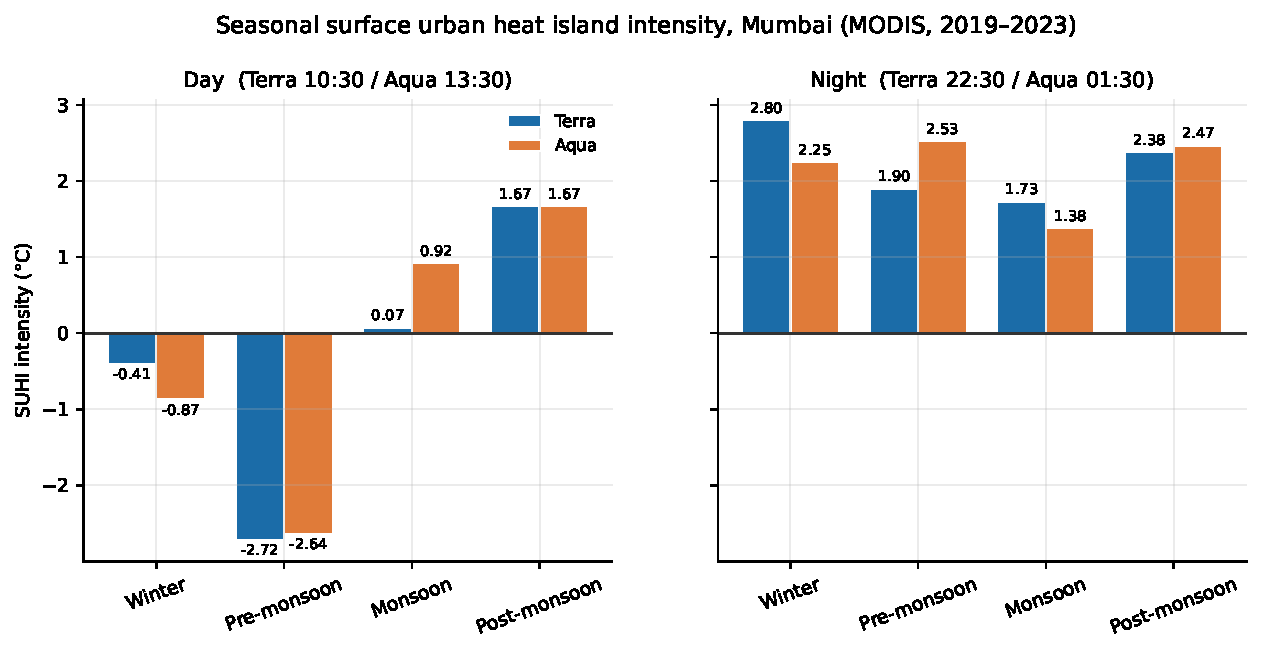
\includegraphics[width=\textwidth]{fig1_seasonal_suhi.pdf}
\caption{Seasonal SUHI for both platforms, day and night.}
\label{fig:seasonal}
\end{figure}

\begin{figure}[htbp]
\centering
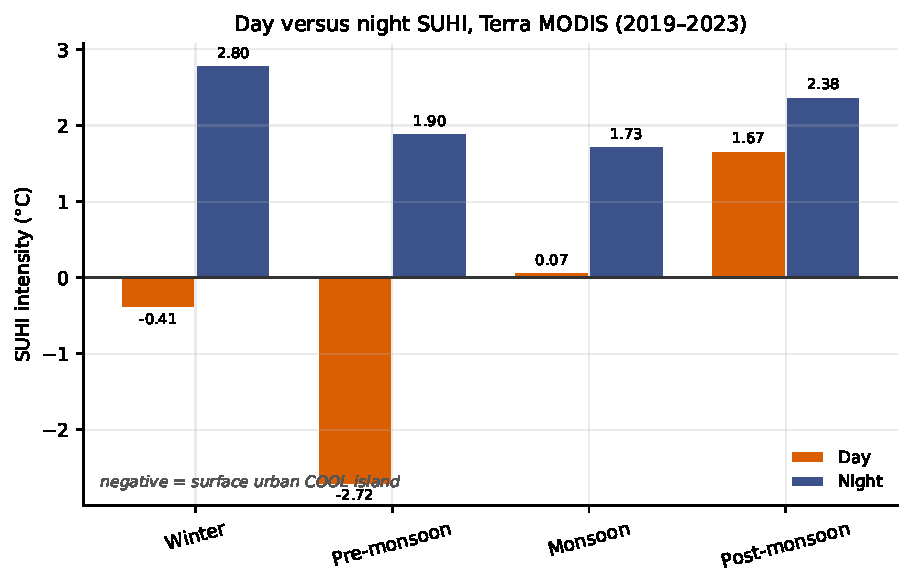
\includegraphics[width=0.8\textwidth]{fig2_day_vs_night.pdf}
\caption{Day and night SUHI side by side, Terra.}
\label{fig:daynight}
\end{figure}

\paragraph{What the numbers show.}
Night-time UHI is positive in every season on both platforms, ranging
from \SI{+1.38}{\degreeCelsius} to \SI{+2.80}{\degreeCelsius}. Daytime
UHI is negative in winter ($-0.41$ Terra, $-0.87$ Aqua) and strongly
negative in pre-monsoon ($-2.72$ Terra, $-2.64$ Aqua), near zero in
monsoon, and positive only in post-monsoon
($+1.67$ on both platforms). A negative value means the rural
surface is hotter than the urban one --- a surface urban \emph{cool}
island.

\TODO{Interpret this. It is the main result of Part~B and carries the
most marks, so it needs several paragraphs of your own reasoning, not
a restatement of the table. Work through at least:

(i) Why is the daytime heat island negative in winter and
pre-monsoon? Look at the urban and rural means separately before
answering --- in pre-monsoon the urban mean is 36.38 and the rural
39.10, so the city has not cooled, the countryside has heated. What
property of a dry bare rural surface would do that, and which thermal
property from the lecture material is doing the work? Thermal inertia
and heat capacity are the relevant ones.

(ii) Why is the night-time island positive in every season when the
daytime one is not? Connect this to what Oke says about UHI being
mostly a nocturnal phenomenon, and to the built-up surface releasing
stored heat after sunset.

(iii) Monsoon daytime UHI is +0.07 (Terra) and +0.92 (Aqua) --- near
zero. What happens to the urban--rural contrast when both surfaces are
wet and evaporating? Note this reading is compromised by the sampling
bias in Section~\ref{sec:sampling}; say so here.

(iv) Terra and Aqua disagree most in monsoon daytime (+0.07 vs +0.92,
a gap of 0.85) and in pre-monsoon night (+1.90 vs +2.53). Since the
only difference is three hours of clock time, what does the size of
that gap tell you about how fast the surface is changing at those
hours?}

\subsection{Clear-sky sampling bias}
\label{sec:sampling}

The monsoon composite is not an average over the monsoon. It is an
average over those monsoon days clear enough for a retrieval to be
produced and pass screening --- which are the least monsoon-like days
of the season.

\begin{table}[htbp]
\centering
\begin{tabular}{lrrr}
\toprule
\textbf{Season} & \textbf{Composites} & \textbf{Mean valid} &
\textbf{Retention} \\
 & \textbf{available} & \textbf{retrievals} & \\
\midrule
Winter       & 40 & 15.6 & 38.9\,\% \\
Pre-monsoon  & 55 & 21.2 & 38.6\,\% \\
Monsoon      & 80 & 10.7 & 13.3\,\% \\
Post-monsoon & 55 & 20.4 & 37.1\,\% \\
\bottomrule
\end{tabular}
\caption{Valid retrievals per pixel against composites available,
Terra day, 2019--2023.}
\label{tab:sampling}
\end{table}

\begin{figure}[htbp]
\centering
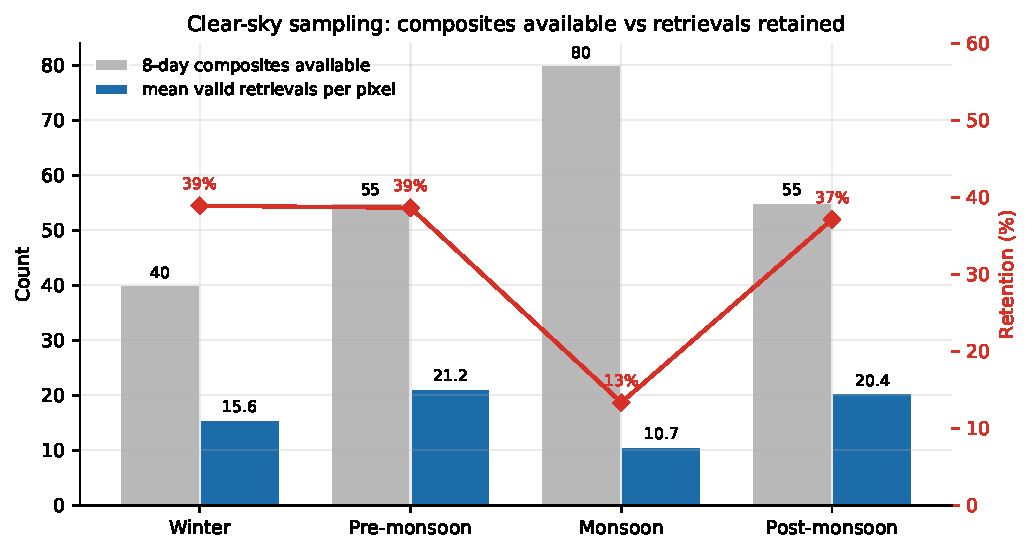
\includegraphics[width=0.8\textwidth]{fig8_sampling_bias.pdf}
\caption{Composites available against retrievals actually retained.
Monsoon has the most input and the fewest usable observations.}
\label{fig:sampling}
\end{figure}

Monsoon has twice as many composites available as winter (80 against
40) but retains the fewest valid retrievals of any season --- 10.7 per
pixel, a retention of 13.3\,\%, against roughly 38\,\% in the other
three seasons.

\TODO{Interpret. Say plainly what the monsoon number therefore
represents, and in which direction it biases the monsoon UHI --- if
the only usable monsoon days are the clear, brighter ones, is the
retrieved monsoon UHI likely too high or too low relative to a true
monsoon average? Then say how much weight the monsoon row in
Table~\ref{tab:headline} deserves because of it.}

\subsection{Urban and rural distributions}

\begin{figure}[htbp]
\centering
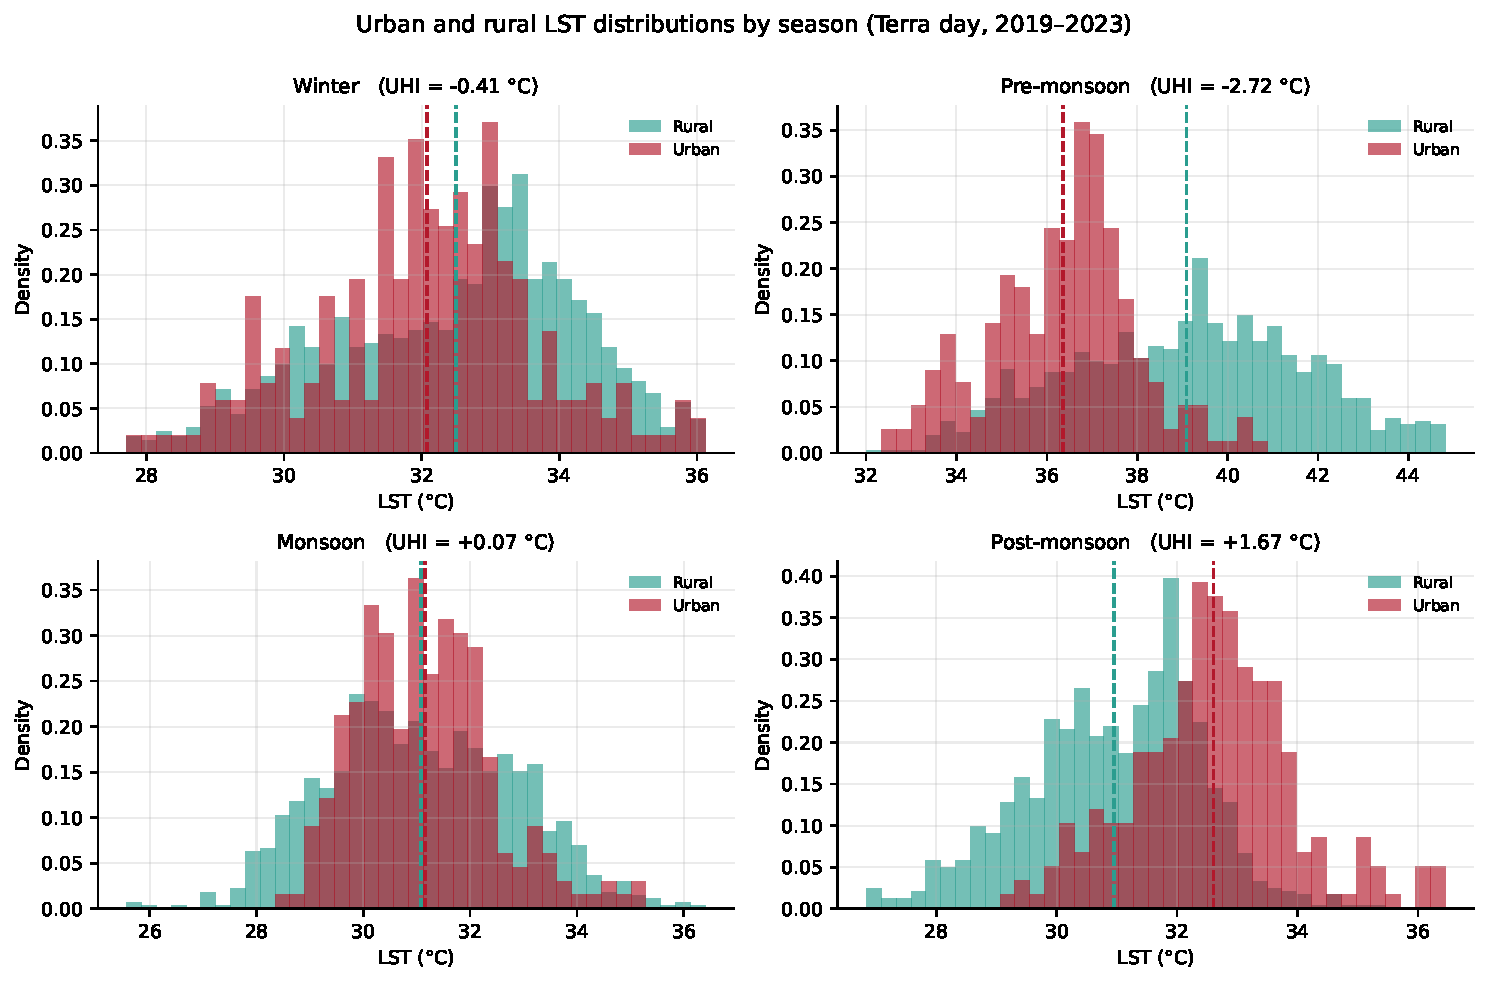
\includegraphics[width=\textwidth]{fig6_distributions.pdf}
\caption{Urban and rural LST distributions by season. Dashed lines
mark the zone means.}
\label{fig:dist}
\end{figure}

\TODO{Interpret. The pre-monsoon panel shows the two distributions
almost fully separated with rural to the right of urban; post-monsoon
shows the reverse with a smaller gap; winter and monsoon overlap
heavily. Address whether the zones separate or merely shift, and note
that the rural distribution is consistently the wider of the two
(rural sd 1.43--3.02 against urban 1.24--1.60 in
Table~\ref{tab:headline}) --- what does a wider rural distribution say
about how mixed that zone is?}

% =============================================================
\section{Sensitivity analysis}
% =============================================================

\subsection{Interannual stability}
\label{sec:interannual}

\begin{table}[htbp]
\centering
\begin{tabular}{lrrrrrr}
\toprule
\textbf{Season} & \textbf{2019} & \textbf{2020} & \textbf{2021} &
\textbf{2022} & \textbf{2023} & \textbf{Range} \\
\midrule
Winter       & $-1.25$ & $-0.27$ & $-0.38$ & $+0.17$ & $-0.30$ & 1.42 \\
Pre-monsoon  & $-3.27$ & $-2.92$ & $-2.74$ & $-2.22$ & $-2.45$ & 1.06 \\
Monsoon      & $+0.06$ & $+1.45$ & $-0.39$ & $-0.31$ & $-0.76$ & 2.20 \\
Post-monsoon & $+1.78$ & $+1.59$ & $+2.01$ & $+1.54$ & $+1.41$ & 0.60 \\
\bottomrule
\end{tabular}
\caption{UHI intensity (\si{\degreeCelsius}) by season and year,
Terra day.}
\label{tab:interannual}
\end{table}

\begin{figure}[htbp]
\centering
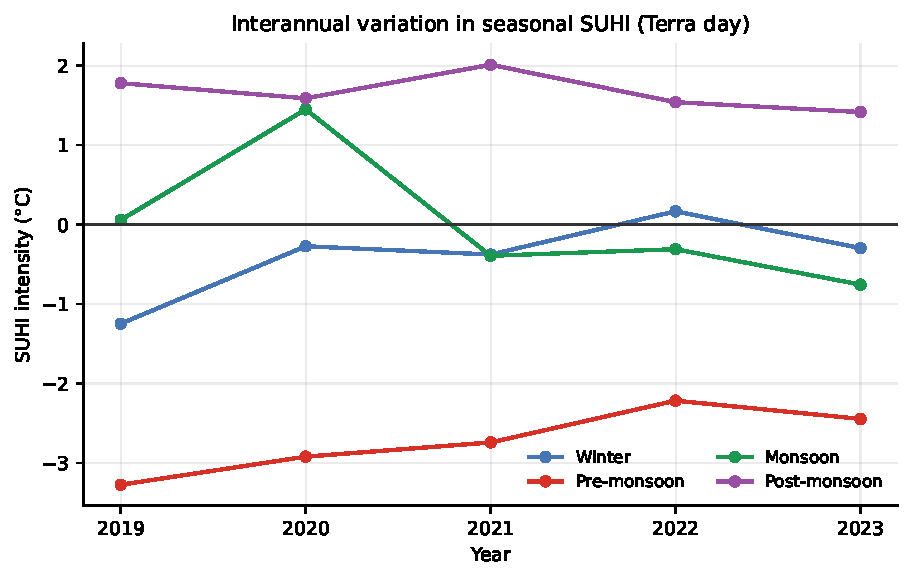
\includegraphics[width=0.8\textwidth]{fig3_interannual.pdf}
\caption{Year-by-year seasonal SUHI, Terra day.}
\label{fig:interannual}
\end{figure}

Pre-monsoon is negative in all five years and post-monsoon positive in
all five. Winter changes sign once (2022, $+0.17$). Monsoon changes
sign three times and has the widest range at
\SI{2.20}{\degreeCelsius}.

\TODO{Interpret. The question is not whether the numbers move but
whether the ordering of the seasons holds in every year --- check that
and state it. Then compare the interannual range against the
between-season differences: pre-monsoon and post-monsoon are separated
by about 4.4\,\si{\degreeCelsius} while their year-to-year ranges are
about 1\,\si{\degreeCelsius} and 0.6\,\si{\degreeCelsius}, whereas
monsoon's range of 2.2\,\si{\degreeCelsius} is larger than its
distance from zero. Say which of the four seasonal results you would
actually stand behind and which you would not, and connect the monsoon
instability back to Section~\ref{sec:sampling}.}

\subsection{Rural ring definition}
\label{sec:ringsens}

\begin{table}[htbp]
\centering
\begin{tabular}{lrrrrr}
\toprule
\textbf{Ring} & \textbf{Winter} & \textbf{Pre-mon.} &
\textbf{Monsoon} & \textbf{Post-mon.} & $n_{\mathrm{rur}}$ \\
\midrule
\SIrange{2}{20}{\kilo\metre}  & $-0.29$ & $-2.55$ & $+0.16$ & $+1.73$ & 1115 \\
\SIrange{5}{20}{\kilo\metre}$^\dagger$ & $-0.41$ & $-2.72$ & $+0.07$ & $+1.67$ & 1055 \\
\SIrange{10}{25}{\kilo\metre} & $-0.58$ & $-3.05$ & $-0.05$ & $+1.65$ &  893 \\
\SIrange{5}{30}{\kilo\metre}  & $-0.40$ & $-2.74$ & $+0.09$ & $+1.70$ & 1055 \\
\midrule
\textbf{Range}                &   0.29  &   0.50  &   0.21  &   0.08  & \\
\bottomrule
\end{tabular}
\caption{UHI (\si{\degreeCelsius}) under four rural ring definitions,
Terra day. $^\dagger$ used for the headline results.}
\label{tab:ringsens}
\end{table}

\begin{figure}[htbp]
\centering
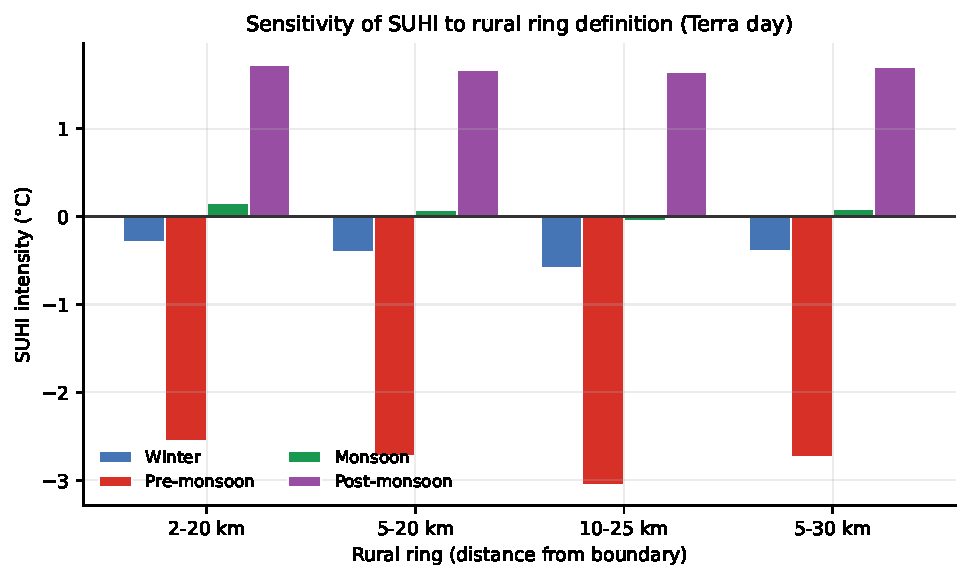
\includegraphics[width=0.85\textwidth]{fig4_ring_sensitivity.pdf}
\caption{SUHI under four rural ring definitions.}
\label{fig:ring}
\end{figure}

Moving the inner edge from \SI{2}{\kilo\metre} to
\SI{10}{\kilo\metre} shifts UHI by up to
\SI{0.50}{\degreeCelsius} (pre-monsoon). Pushing the outer edge from
\SI{20}{\kilo\metre} to \SI{30}{\kilo\metre} changes almost nothing
(\SI{0.01}{\degreeCelsius} to \SI{0.03}{\degreeCelsius}).

\TODO{Interpret. Two things to address. First, the direction: as the
inner edge moves outward the rural mean rises and UHI becomes more
negative in every season --- what does a rural reference that keeps
getting hotter the further you go from the city imply about how far
the city's influence reaches, and does that support or undermine the
5\,km gap we chose? Second, the outer edge barely matters while the
inner edge does; what does that asymmetry tell you about where the
useful rural land actually sits? Finally, compare the ranges here
(0.08--0.50\,\si{\degreeCelsius}) against M's identical sweep on
Landsat --- both use the same ring function, so they are directly
comparable --- and explain any difference in terms of pixel size.}

\subsection{Water in the rural reference}
\label{sec:watertest}

We recomputed UHI with water, wetland and mangrove left in the rural
reference, holding everything else fixed.

\begin{table}[htbp]
\centering
\small
\begin{tabular}{llrrr}
\toprule
\textbf{Mode} & \textbf{Season} & \textbf{Water excl.} &
\textbf{Water incl.} & \textbf{Difference} \\
\midrule
Day   & Winter       & $-0.41$ & $-0.12$ & $+0.291$ \\
Day   & Pre-monsoon  & $-2.72$ & $-2.28$ & $+0.445$ \\
Day   & Monsoon      & $+0.07$ & $+0.25$ & $+0.176$ \\
Day   & Post-monsoon & $+1.67$ & $+1.77$ & $+0.104$ \\
\midrule
Night & Winter       & $+2.80$ & $+2.80$ & $-0.004$ \\
Night & Pre-monsoon  & $+1.90$ & $+1.93$ & $+0.031$ \\
Night & Monsoon      & $+1.73$ & $+1.64$ & $-0.087$ \\
Night & Post-monsoon & $+2.38$ & $+2.35$ & $-0.035$ \\
\bottomrule
\end{tabular}
\caption{Effect of retaining water in the rural reference, Terra.
All values \si{\degreeCelsius}.}
\label{tab:watertest}
\end{table}

\begin{figure}[htbp]
\centering
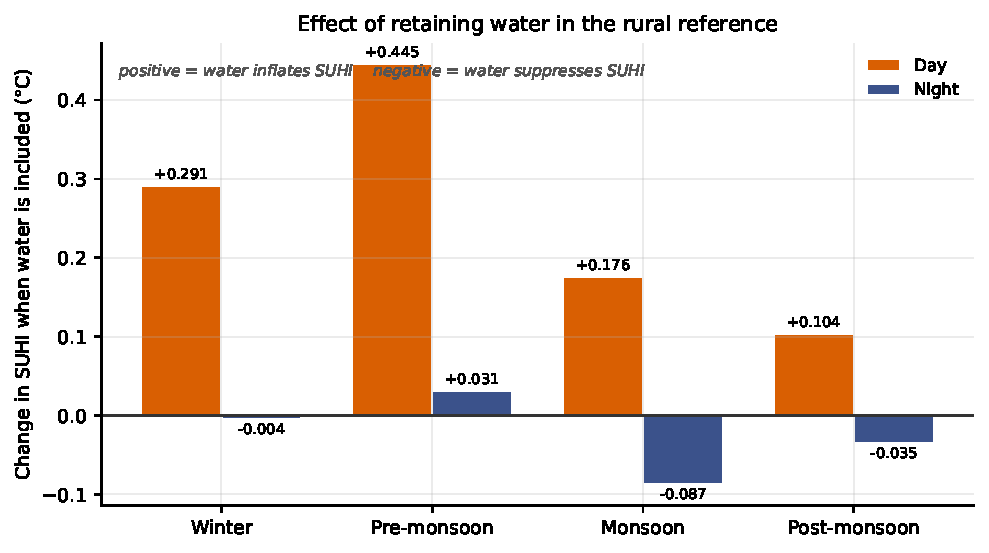
\includegraphics[width=0.85\textwidth]{fig5_water_test.pdf}
\caption{Change in SUHI when water is retained in the rural zone.}
\label{fig:water}
\end{figure}

Every daytime difference is positive (\num{+0.10} to \num{+0.45}).
Three of four night-time differences are negative
(\num{-0.004} to \num{-0.087}).

\TODO{Interpret. This is the test that justifies the exclusion in
Section~\ref{sec:waterexcl}, so tie the two together. The prediction
was that including water would inflate daytime UHI and suppress
night-time UHI, because the sea is cooler than land by day and warmer
by night. State whether the signs in Table~\ref{tab:watertest} bear
that out. Then note that the daytime effect (up to
0.45\,\si{\degreeCelsius}) is roughly five times the night-time effect
(up to 0.09\,\si{\degreeCelsius}), and explain why --- what is the
day--night temperature range of the sea compared with that of land?
Finally, say whether an error of this size would have changed any
conclusion in Section~4.1, and whether that makes the exclusion
necessary or merely tidy.}

% =============================================================
\section{Comparison with the Landsat result}
\label{sec:comparison}
% =============================================================

The overlapping season is post-monsoon: the Landsat pair in Part~A was
acquired on 8--9~October~2015.

\paragraph{Matching in time.}
The headline MODIS figures are 2019--2023 means and the Landsat
observation is a single day in 2015. Comparing them directly would mix
the sensor difference with eight years of urban growth and
year-to-year variation. We therefore recomputed post-monsoon for 2015
alone. Both are reported below: the gap between the two MODIS rows is
interannual variation, and the gap between the matched MODIS row and
the Landsat row is what the sensor comparison is actually about.

\begin{table}[htbp]
\centering
\small
\begin{tabular}{lllrrr}
\toprule
\textbf{Sensor} & \textbf{Period} & \textbf{Mode} &
\textbf{Obs.\ time} & \textbf{Res.} & \textbf{UHI} \\
 & & & (local) & (\si{\metre}) & (\si{\degreeCelsius}) \\
\midrule
Landsat 8 & 8 Oct 2015 & Day   & \TODO{from M} & 30 & \TODO{from M} \\
Landsat 8 & 9 Oct 2015 & Night & \TODO{from M} & 30 & \TODO{from M} \\
\midrule
Terra & 2015      & Day   & 10:41 & 1000 & $+1.24$ \\
Terra & 2019--23  & Day   & 10:32 & 1000 & $+1.67$ \\
Aqua  & 2015      & Day   & 13:24 & 1000 & $+1.71$ \\
Aqua  & 2019--23  & Day   & 13:32 & 1000 & $+1.67$ \\
\midrule
Terra & 2015      & Night & 22:19 & 1000 & $+2.09$ \\
Terra & 2019--23  & Night & 22:09 & 1000 & $+2.38$ \\
Aqua  & 2015      & Night & 01:49 & 1000 & $+2.36$ \\
Aqua  & 2019--23  & Night & 01:53 & 1000 & $+2.47$ \\
\bottomrule
\end{tabular}
\caption{Post-monsoon UHI. The 2015 rows are matched to the Landsat
acquisition year.}
\label{tab:comparison}
\end{table}

\begin{figure}[htbp]
\centering
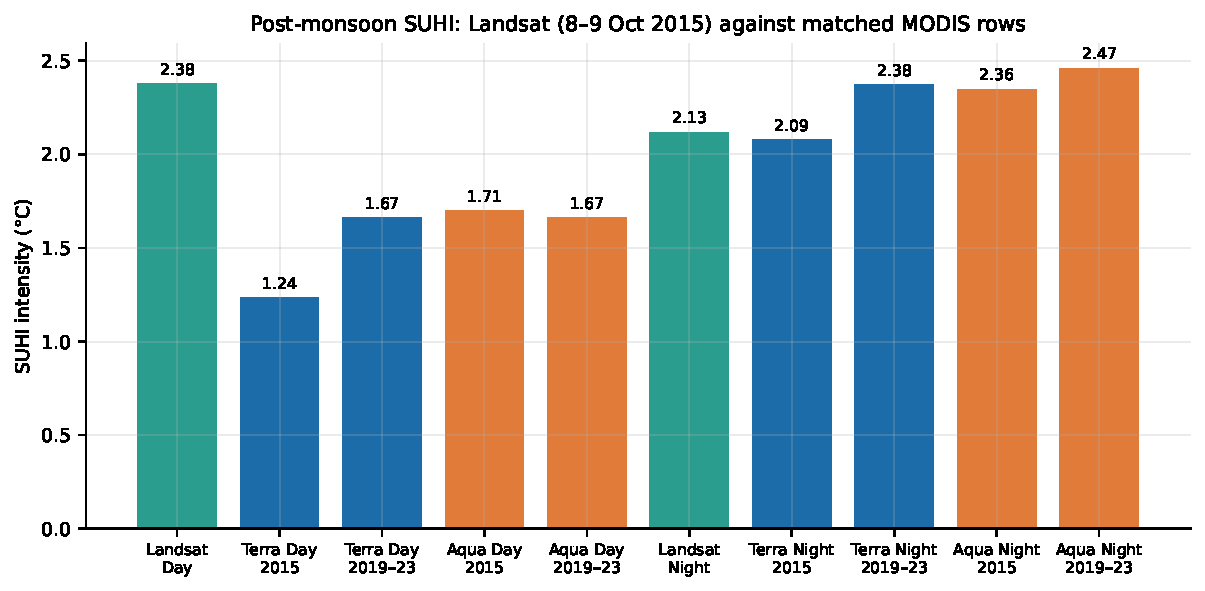
\includegraphics[width=0.85\textwidth]{fig7_cross_sensor.pdf}
\caption{MODIS post-monsoon SUHI, 2015 against the 2019--2023 mean.
M's Landsat bars to be added.}
\label{fig:cross}
\end{figure}

\paragraph{Brightness temperature against LST.}
Part~A reports night-time \emph{brightness temperature}, not LST,
because no emissivity correction was applied. MODIS night LST is
emissivity-corrected. Brightness temperature is lower than LST
wherever \(\varepsilon < 1\), and the offset differs between built-up
(\(\varepsilon \approx 0.97\)) and vegetated
(\(\varepsilon \approx 0.98\)--\(0.99\)) surfaces, so it does not
cancel in the urban-minus-rural subtraction. This has to be stated
wherever the night rows are compared.

\TODO{Account for the disagreement once M's numbers are in. Four
mechanisms are available and they should be weighed, not just listed:

\begin{enumerate}
  \item \textbf{Resolution.} A \SI{1}{\kilo\metre} MODIS pixel over
  Mumbai mixes built-up with vegetation, water and open ground, which
  compresses the urban--rural contrast. MODIS UHI should therefore be
  \emph{smaller} than Landsat. If your numbers show otherwise, that
  needs explaining rather than glossing.
  \item \textbf{Overpass time.} Terra day and Landsat day are within
  about eight minutes. Use the Terra--Aqua gap in
  Table~\ref{tab:comparison} to put a number on how much three hours
  of clock time is worth, then judge how much of the Landsat--MODIS
  gap time of day can account for.
  \item \textbf{Temporal sampling.} Landsat is one instantaneous scene
  carrying that day's weather; the matched MODIS row is a three-month
  seasonal mean for the same year. Note that post-monsoon runs
  October--December while M's scene is 8 October, so even the matched
  row averages two months the Landsat scene does not see.
  \item \textbf{Retrieval and emissivity.} MOD11A2 uses a split-window
  with land-cover-class emissivity; Landsat Collection~2 uses a
  single-channel retrieval with ASTER-GED emissivity. The lecture
  material gives roughly \SI{1}{\kelvin} of LST error per
  \SI{1.5}{\percent} of emissivity error, so this is not negligible.
\end{enumerate}

Rank these and say which you think dominates for your case.}

\paragraph{Zone definitions.}
\TODO{Part A currently uses non-built pixels inside the city as its
rural reference, while Part B uses the external 5--20\,km ring. The
brief requires both parts to share one definition. Record here what
was agreed and which numbers were recomputed.}

% =============================================================
\section{Additional findings}
% =============================================================

\TODO{Optional but marked. The strongest candidate is already in your
data: the day--night reversal. Daytime UHI is negative in two seasons
while night-time UHI is positive in all four, which is the nocturnal
dominance described by Oke appearing in your own measurements, and it
links Part~B straight to Part~A's day/night contrast.

Two others worth computing if there is time. Urban minus rural diurnal
range (day LST minus night LST per zone) would test whether the
built-up surface has the narrower range, which is the apparent thermal
inertia argument from the lecture material --- the numbers for this
are already in Table~\ref{tab:headline}. Mean LST by WorldCover class
would show which covers actually drive the urban mean.}

% =============================================================
\section*{References}
% =============================================================

\begin{thebibliography}{9}

\bibitem{imd_seasons}
\TODO{India Meteorological Department reference for the four-season
classification. Title, URL, access date.}

\bibitem{gadm}
Global Administrative Areas (2022) \textit{GADM database of Global
Administrative Areas, version 4.1}. Available at:
\url{https://gadm.org/data.html} (Accessed: \TODO{date}).

\bibitem{mod11a2}
Wan, Z., Hook, S. and Hulley, G. (2021) \textit{MODIS/Terra Land
Surface Temperature/Emissivity 8-Day L3 Global 1km SIN Grid V061}.
NASA EOSDIS Land Processes DAAC. \TODO{DOI and access date.}

\bibitem{myd11a2}
Wan, Z., Hook, S. and Hulley, G. (2021) \textit{MODIS/Aqua Land
Surface Temperature/Emissivity 8-Day L3 Global 1km SIN Grid V061}.
NASA EOSDIS Land Processes DAAC. \TODO{DOI and access date.}

\bibitem{worldcover}
Zanaga, D. \textit{et al.} (2022) \textit{ESA WorldCover 10 m 2021
v200}. \TODO{DOI and access date.}

\bibitem{oke}
Oke, T.R., Mills, G., Christen, A. and Voogt, J.A. (2017)
\textit{Urban Climates}. Cambridge: Cambridge University Press.

\end{thebibliography}

% =============================================================
\section*{Appendix: Earth Engine script}
% =============================================================

Part~B script (view access):\\
\url{https://code.earthengine.google.com/f00b8b3999cd01e32f97a9d001740569}

% =============================================================
\section*{Declaration on the use of AI tools}
% =============================================================

\TODO{Write this yourself, and be specific. It has to say which tools
were used and for what. The brief allows AI for explaining concepts,
debugging code you wrote, and improving the clarity of prose, but not
for generating the justifications or the interpretation --- so those
sections must be your own, and the declaration should say so.}

\end{document}
